\documentclass[11pt]{llncs}

\usepackage{graphicx} 
\usepackage{natbib}
\usepackage[utf8]{inputenc}

\title{Das \\ Flussproblem}

\author{Jan Niklas Hollenbeck \\ und \\ Marco Leeske}

\date{\today}

\begin{document}

\maketitle

\newpage

\begin{abstract}

In diesem Paper wird das Flussproblem beleuchtet, welches ein mathematisches Problem zur Findung des maximalen Flusses in Netz\-werken beschreibt.
 Probleme des realen Lebens, beispielsweise in Kanal- oder Verkehrsleitsystemen, werden als gerichtete Graphen mo\-delliert und mittels Algorithmen gelöst.
 Zur Lösung des Flussproblems gibt es unterschiedliche Algorithmen, welche sich in Laufzeit und Anwendungsfall unterscheiden.
 Die vorliegende Arbeit soll einen Überblick über zwei verschiedene Algorithmen sowie deren Anwendungsbereiche geben, um die Auswahl, des optimalen Algorithmus für den jeweils vorliegenden Anwendungsfall, zu erleichtern.
 Es werden die Funktionsweisen der Algorithmen von Ford und Fulkerson sowie Edmond und Karp erläutert, empirisch untersucht und es wird ein Laufzeitvergleich durchgeführt.
 Dies wird mit Hilfe eines Java Programmes, welches für jeden Datensatz alle Algorithmen testet, realisiert.
Es werden die jeweiligen Vor- und Nachteile der Algorithmen aufgezeigt, der Funktionsumfang geprüft und anschließend die gesammelten Resultate der Laufzeittests verglichen, um sowohl eine Übersicht als auch eine Entscheidungshilfe geben zu können.
 Die Frage, welcher Algorithmus bei unterschiedlichen Ausgangssituationen und Erwartungen den Vorzug erhält, wird sich nach der Lektüre dieser Arbeit beantworten lassen. 

\end{abstract}


\section{Einleitung}
\label{Einleitung}

Das wird die Einleitung. Das wird die Einleitung. Das wird die Einleitung. Das wird die Einleitung. Das wird die Einleitung. Das wird die Einleitung. Das wird die Einleitung. Das wird die Einleitung. Das wird die Einleitung. Das wird die Einleitung. Das wird die Einleitung. Das wird die Einleitung. Das wird die Einleitung. Das wird die Einleitung. Das wird die Einleitung. Das wird die Einleitung. Das wird die Einleitung. Das wird die Einleitung. Das wird die Einleitung. Das wird die Einleitung. Das wird die Einleitung. Das wird die Einleitung. Das wird die Einleitung. Das wird die Einleitung. Das wird die Einleitung. Das wird die Einleitung. Das wird die Einleitung. Das wird die Einleitung. Das wird die Einleitung. Das wird die Einleitung. Das wird die Einleitung. Das wird die Einleitung. Das wird die Einleitung. Das wird die Einleitung. Das wird die Einleitung. 

%\newpage
%\tableofcontents

\newpage
\section{Einführung}
\label{Einfuehrung}
Das Flussproblem beschreibt ein mathematisches Problem in Netzwerken.

\subsection{Algorithmus}
\label{Algorithmus}
Ein Algorithmus beschreibt eine Handlungsvorschrift zur Abarbeitung eines Problems in Einzelschritten, welches mittels Algorithmen lösen lässt. 

\subsection{Algorithmus von Ford und Fulkerson}
Beschreibung und Erläuterung des Ford und Fulkerson Algorithmus

\subsection{Algorithmus von Edmonds und Karp}
Beschreibung und Erläuterung des Edmond und Karp Algorithmus

\subsection{Netzwerke}
\label{Netzwerke}
Systeme deren Struktur sich als mathematischer Graph darstellen lassen


\subsection{Gerichteter Graph}
\label{Graph}
Ein gerichteter Graph ist ein Objekt aus der mathematischen Graphentheorie.


\begin{figure}[htbp] 
  \centering
     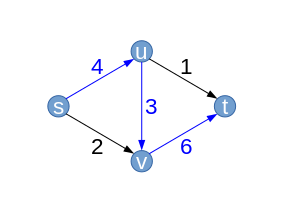
\includegraphics{graph1} 
  \caption{Bild eines Netzwerk-Graphen}
  \label{fig:Graph1}
\end{figure}


\section{Der Inhalt}
\label{Inhalt}

Flussprobleme k\"onnen in Netzwerken mithilfe von Graphen modelliert werden. Hierbei ist ein Quelle-Senke-Netzwerk(im Folgenden q-s-Netzwerk) ein kantenbewerteter, gerichteter Graph G = (V, E) mit der Eigenheit, dass eine Ecke q als Quelle sowie eine Ecke s als Senke bezeichnet wird. Die zwischen Quelle und Senke liegenden Knoten und Kanten können als Zwischenstationen aufgefasst werden. \"Uberdies wird jeder Kante, also eine Verbindung von zwei Ecken im Netzwerk, eine Kapazität c zugewiesen. Sie gibt an, wie viel maximal durch die Kante fließen kann. \citep{Testref}

In Figure \ref{fig:Graph1} unter \ref{Graph} sieht man die Senke auf der linken Seite, gekenn-zeichnet durch "S". 



\section{Experimente}
\label{Experimente}

\subsection{Wirkungsweise der Algorithmen}

\subsection{Laufzeitvergleich}

\subsection{Anwendungszenarien der jeweiligen Algorithmen}

\section{Stand der Technik (Related Work)}
\label{Related Work}
\subsection{Algorithmen und Datenstrukturen Springer Verlag}
\subsection{Graphentheoretische Konzepte und Algorithmen Vieweg und Teubner}

\section{Zusammenfassung}
\label{Zusammenfassung}
\subsection{Ausblick}



\bibliography{test}
\bibliographystyle{plainnat} 

\end{document}
